\documentclass[10pt,twocolumn]{article}
\usepackage[margin=0.75in]{geometry}
\usepackage[T1]{fontenc}
\usepackage{lmodern,amsmath,amssymb,booktabs,graphicx,hyperref,microtype}
\hypersetup{colorlinks=true,urlcolor=blue,linkcolor=blue}
\newcommand{\StructureCount}{3}
\newcommand{\EpisodeCount}{12}
\newcommand{\ProbeCount}{39}
\newcommand{\StateCount}{342,704}
\newcommand{\EdgeCount}{2,843,080}
\newcommand{\AirframeActions}{21}
\newcommand{\AirframeChain}{5}
\newcommand{\AirframeSourceChain}{3 $\rightarrow$ 8 $\rightarrow$ 16 $\rightarrow$ 30 $\rightarrow$ 32}
\newcommand{\SemanticTests}{17}
\newcommand{\RemovedParts}{P008, P012, P019}
\newcommand{\InsertedPart}{P002}
\newcommand{\InsertionSite}{S021}
\newcommand{\RepairActions}{10}

\title{BrickPlan 1.1: Certified Assembly-Order Diagnostics\\Across Two Source Families}
\author{Executable benchmark release}
\date{October 2, 2026}
\begin{document}
\maketitle
\begin{abstract}
A correctly placed part can obstruct a future insertion and force removal.
BrickPlan diagnoses this planning failure with locally goal-independent actions,
exact future-feasibility labels, and auditable recovery costs. Version 1.1 extends
the frozen 1.0 bank with an original airframe subassembly from a second source
kit. The bank contains \StructureCount{} structures, \EpisodeCount{} episodes,
and \ProbeCount{} diagnostic responses, covering \StateCount{} reachable states
and \EdgeCount{} directed transitions. The new structure requires
\AirframeActions{} attachments from its fixed base and has an exact mandatory
chain of \AirframeChain{} parts across all detach-free completions.
Seven dimensions measure dead-end choices, supplied-plan conflict prediction,
plan survival, regret, recovery, replanning efficiency, and counterfactual
consistency. Every injected repair requires three removals. A shared HTTP
executor supports human practice, model clients, and original-mesh 3D replay.
Results below are software validation controls; no model or human performance
has been measured.
\end{abstract}

\section{Problem and contribution}
Assembly planning must maintain object identities, support, access paths, and
future requirements across many individually plausible actions. Closing a region
early may execute successfully while making every remaining attachment-only
completion impossible. End-to-end success cannot distinguish this event from
an immediately invalid action or an inaccurate pose.

LEGO-Puzzles motivates multistep planning evaluation~\cite{legopuzzles};
PhyBlock studies physical planning~\cite{phyblock}; Brick-Composer studies
fine-grained selection and placement~\cite{composer}. Their reported metrics
measure different outcomes and are not interchangeable episode success rates.
Interactive assembly and reconstruction also precede this benchmark, including
LTRON~\cite{ltron} and InstructioNet~\cite{instructionet}.
The contribution here is an executable measurement contract connecting
decisions, feasibility loss, diagnosis, and recovery to exact finite-domain
certificates. It is not a claim that interaction or disassembly is new.

The extension addresses two concrete limitations of 1.0: its two structures
shared one source kit, and both mandatory chains contained four parts.
The airframe adds a separate kit and a longer certified order. Two provenance
groups still do not establish broad generalization, and a deeper mandatory
assembly chain does not establish deeper conflict-probe causality.

\section{Workcell and certified bank}
\subsection{Action and observation contract}
Each task supplies a connected, clamped fixed base, an inventory, calibrated
sites, and a visible exact target. Original source geometry and placements are
preserved. Attach and detach move one part along its declared straight path.
Every accepted state remains connected to the fixed base through audited stud
connections, abstracted as rigid holds. External magazine transfer, hands,
grasping, clutch force, and gravity are outside the certified domain.

Local legality depends only on current occupancy, path obstruction, and support.
The executor does not consult the future goal or cost oracle. Thus a legal
closure that causes later rework actually executes. The goal requires exact
occupancy, including removal of extra parts. All sites remain selectable;
there is no next-step feasibility mask. Structural attempts cost one action,
including rejected attempts; inspection and diagnosis have separate quotas.

Public part and site IDs are stable within an episode and randomized by seed.
Equivalent parts of the same type and color are exchangeable. Observations
provide source geometry in calibrated coordinates but exclude instruction
indices, blocker tables, oracle costs, viability, and reference actions.
The browser adds camera control and an exploded reference for practice and
review. Actual assembly states retain their source poses.

\subsection{Geometry and provenance}
Display uses original recursively resolved LDraw triangles. Collision proxies
are closed meshes inset by 0.25 LDU per surface, with a 0.002 LDU guard.
All final-pose pairs must be clear. Each moving part is checked against every
other included part across its full declared translation. Separating swept
bounds certify easy clear pairs; otherwise midpoint separation $d$ certifies
an interval $[l,h]$ when $d>(h-l)/2+0.002$, by the 1-Lipschitz property of
surface distance under unit translation. Triangle intersections provide blocked
witnesses. Unresolved coverage is UNKNOWN and excludes the candidate.

The inherited 3022 collision-proxy repair fills one source-verified missing
triangular stud-cap face without moving vertices. Original render meshes remain
unchanged. These are numerical certificates for the declared proxy/path domain,
not guarantees for unrestricted six-degree-of-freedom manipulation.

\begin{table*}[t]
\centering\small
\caption{Frozen case bank. Roadster and kart share LEGO 31027; airframe is from
LEGO 31028. Counts describe separate state graphs, not independent trials.}
\begin{tabular}{llrrrrrr}\toprule
Case & Source group & Fixed/movable & States & Directed edges & Full actions & Chain parts & Repair detaches\\\midrule
Roadster & LEGO-31027 & 20/17 & 14,012 & 131,824 & 17 & 4 & 3\\
Kart & LEGO-31027 & 7/18 & 44,604 & 436,824 & 18 & 4 & 3\\
Airframe & LEGO-31028 & 3/21 & 284,088 & 2,274,432 & 21 & 5 & 3\\
\bottomrule\end{tabular}

\label{tab:cases}
\end{table*}

The airframe selects source instances 0--34 excluding 11--14 and 21--27;
instances 1, 2, and 5 form its fixed base. The propeller, float/clip assemblies,
and main wing plates are outside this fuselage, tail and upper-plate subassembly.
The 54383/54384 wing proxies contain extensive nonmanifold and boundary edges;
both wings and their dependent top plate are excluded without proxy repair.
Every included endpoint and
motion pair is requalified; earlier exploratory sampled paths are not accepted
as ground truth. The exact new mandatory chain is \AirframeSourceChain{}
in private source-index notation. These source indices never enter policy
observations.

\subsection{Exact finite-domain labels}
Let $s$ encode occupied mutable sites and $g$ the exact goal. Exhaustive search
enumerates the reachable component; goal-rooted breadth-first search computes
$C^*(s,g)$, the minimum successful unit-action count. Every edge has a verified
inverse. For every stored goal, Bellman inequalities, unique zero-cost
termination, component equality, and decreasing successors certify the table.
Geometry, source, transition, task, and cost hashes identify the release.

If $\Delta=|g|-|s|$, successful one-part actions satisfy
attachments minus detachments $=\Delta$. Therefore
\[
D^*(s,g)=(C^*(s,g)-\Delta)/2.
\]
No-undo feasibility is $V^+(s,g)=[s\subseteq g \land C^*(s,g)=\Delta]$;
budget feasibility is $V_B(s,g,b)=[C^*(s,g)\le b]$.
A no-undo dead end is recoverable with removal, not absolute impossibility.

Mandatory precedence is the intersection of ordering constraints over
\emph{all} detach-free full completions. A source pair $i\prec j$ is mandatory
only if no viable detach-free prefix contains $j$ without $i$.
The longest chain in this relation is separate from total task length and
from the first-conflict distance of a supplied plan.

\subsection{Episodes and paired probes}
Each structure supplies full, checkpoint, repair, and matched healthy episodes.
Checkpoints are at least three successful actions from the fixed base and offer
both safe and costly locally legal continuations. Repair starts are reachable and require exactly
three detachments. Healthy controls match installed count and inherit the
repair budget. Default budgets are $C^*+\max(4,\lceil C^*/2\rceil)$.

Per structure, one choice probe evaluates a legal decision at a tight budget;
eight lookahead probes cover distances 1, 2, 4, and 8 with executable controls;
four counterfactual members form a switching pair and an invariance pair.
All starts have reachability witnesses, and all episode completions have
optimal action witnesses. Random IDs and repeated runs do not create new
independent structures.

\section{Seven diagnostic dimensions}
\paragraph{Dead-end choice rate.}
Among eligible legal choices with feasible predecessors, count losses of
$V^+$, and separately losses of $V_B$ after decrementing the budget. Missing,
invalid, and valid responses have separate counts; all-assigned avoidance
prevents abstention from earning full credit.

\paragraph{Lookahead depth.}
Predict the first failing action index of a supplied continuation, or null
when all actions execute. Report exact accuracy, conflict recall, false alarms,
and coverage by distance. The causal depth of these obstruction probes remains
\emph{one}, including in 1.1. Longer bins contain intervening legal attachments.
An executable control need not preserve eventual goal feasibility.
This measures a conflict-prediction curve, not internal search depth.

\paragraph{Plan survival.}
Freeze the first attempted-action index losing each feasibility predicate;
later recovery never erases the loss. For $N$ initially eligible runs, report
known survivors $A_t$ and unresolved early stops $U_t$ with bounds
$[A_t/N,(A_t+U_t)/N]$. Completed successes are absorbing, while abandoned
runs are not assumed to survive indefinitely. Stratify by case and mode.

\paragraph{Regret.}
Successful action regret is attempted actions minus $C^*(s_0,g)$;
detach regret is detach operations minus $D^*(s_0,g)$.
Failed or unfinished runs have null regret and explicit consumed costs.
In this domain, action regret equals twice detach regret plus failed attempts;
these are related cost measures.

\paragraph{Recovery rate.}
Score the first explicit needs-rework diagnosis before the first successful
structural action. Prior failed attempts are separately flagged. Report
detection recall, precision, healthy false alarms, recovery completion, and
joint detection/completion. Later diagnoses cannot replace the first answer.

\paragraph{Replanning efficiency.}
Report detaches, distinct removed instances, wasted attempts, regret, and the
first useful repair reducing $D^*$. Conditional efficiency accompanies
completion rate; self-induced and injected recovery states remain distinct.

\paragraph{Counterfactual consistency.}
Hold state, inventory, sites, paths, and two offered closures fixed while
changing the visible goal. Both closures remain required. Exact conditional
costs $Q^*(s,a,g)=1+C^*(T(s,a),g)$ determine the best \emph{offered} choice.
Switch pairs reverse the unique minimizer; invariance pairs retain it.
Score joint correct switching and correct invariance after depermuting
candidate positions. A globally better interior insertion may exist outside
the two offered actions.

\section{Validation and experimental settings}
Complete success at the frozen budget is the headline outcome; no weighted
composite is defined. The unchanged 1.0 engine and metric implementation are
bound to the extended bank through a release-specific entry point. Old files
remain frozen dependencies. The new launcher stamps collected metadata and
evaluation output with the benchmark version. HTTP requests are revision
checked, idempotent, and atomically journaled. Terminal-only exports are replayed
authoritatively before scoring.

\begin{table}[t]
\centering\small
\caption{Privileged software controls; not model or human results.}
\begin{tabular}{lrr}\toprule
Controller & Complete & Repair\\\midrule
Optimal oracle & 12/12 & 3/3\\
Fault + recovery & 12/12 & 3/3\\
Trap + attach only & 3/12 & 0/3\\
\bottomrule\end{tabular}

\end{table}

\SemanticTests{} semantic tests verify complete cost tables, mandatory
precedence, source preservation, proof tampering, invalid inputs, missing
responses, censoring, wrong switching, budget exhaustion, identity, and diagnosis
timing. HTTP validation completes \EpisodeCount{} episodes and \ProbeCount{}
responses, then checks restart, collection, scoring, and private-route rejection.
Browser validation executes full and repair episodes for every structure
through actual buttons, including a charged incompatible-part attempt in each
full episode. It verifies replay, downloads, displayed-probe identity, and
desktop/mobile layout.

\begin{figure*}[t]
\centering
\begin{minipage}{.48\textwidth}\centering
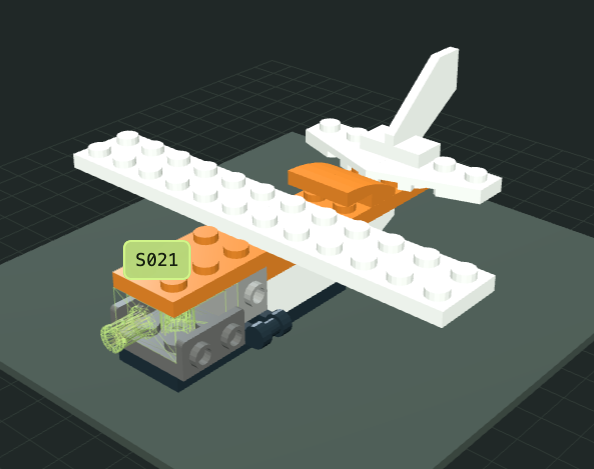
\includegraphics[width=\linewidth]{figures/repair-0-detail.png}\\
\small (a) Reachable repair start.
\end{minipage}\hfill
\begin{minipage}{.48\textwidth}\centering
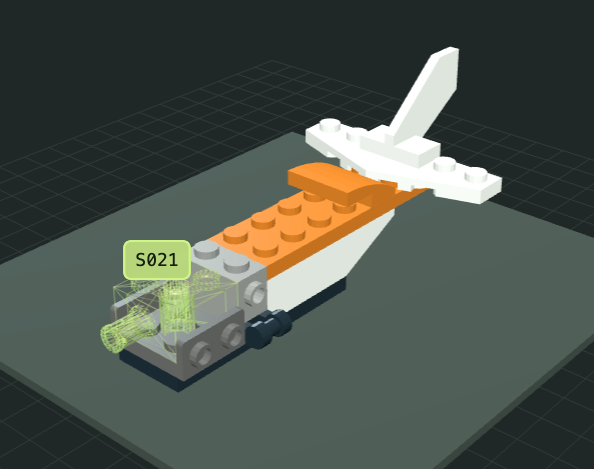
\includegraphics[width=\linewidth]{figures/repair-1-detail.png}\\
\small (b) Three removals completed.
\end{minipage}

\medskip
\begin{minipage}{.48\textwidth}\centering
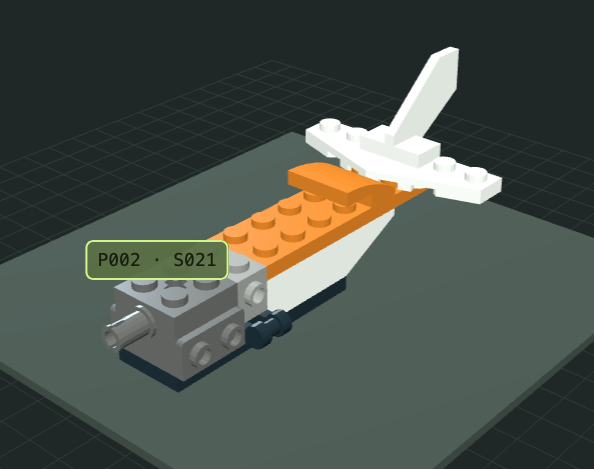
\includegraphics[width=\linewidth]{figures/repair-2-detail.png}\\
\small (c) Install the interior part.
\end{minipage}\hfill
\begin{minipage}{.48\textwidth}\centering
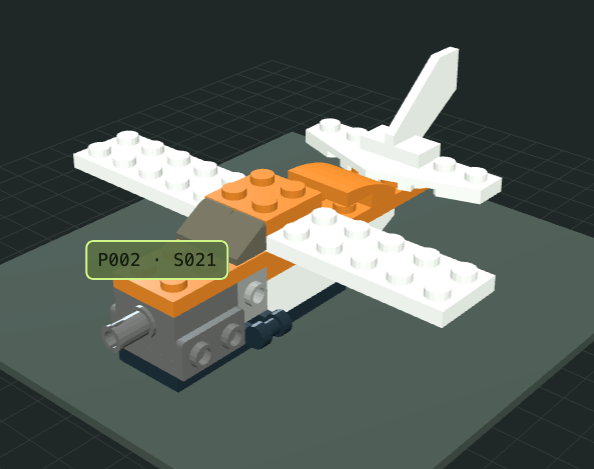
\includegraphics[width=\linewidth]{figures/repair-3-detail.png}\\
\small (d) Restore the target.
\end{minipage}
\caption{Actual airframe repair replay, seed 31. Remove \RemovedParts{},
then install \InsertedPart{} at \InsertionSite{} and restore the target.
The complete recovery uses \RepairActions{} successful actions and exactly
three detachments, matching the certified optimum. Empty-site wireframes are
locators, not installed floating parts. Frames come from authoritative executor
states rendered with original LDraw triangles; only screenshot margins are cropped.}
\end{figure*}

\begin{table}[t]
\centering\small
\caption{Preregistered study framework; empirical slots remain unfilled.}
\begin{tabular}{ll}\toprule
Condition & Status\\\midrule
Model: stepwise structured policy & Not evaluated\\
Same model: explicit planning & Not evaluated\\
Human structured protocol & Not evaluated\\
Matched image-only observations & Not implemented\\\bottomrule
\end{tabular}
\end{table}

Before a model study, specify exact model/provider/version, prompts, token and
context budgets, reasoning settings, observation access, seeds, retry policy,
costs, and selection among repeated runs. Isolate the policy process from
private certificate files and post-trial oracle tools. Split by source family;
roadster and kart must remain together. Two source groups are insufficient for
strong population-level confidence statements.

\section{Limitations}
The new case strengthens provenance coverage and mandatory dependency length,
but all full episodes remain short diagnostic builds in the proposed D1 range.
The supplied-plan obstruction probes still have causal depth one. No maximum
reasoning horizon, 100-step planning, VLM perception, or human advantage is
established. Known poses, fixed straight paths, rigid stud support, and inset
meshes restrict physical validity. Alternative insertion directions, simultaneous
subassembly motion, free rotation, calibrated clutch forces, hand access, and
physical construction remain unverified. The next empirical question is whether
these diagnostics explain model failures beyond immediate action errors.

\begin{thebibliography}{9}\small
\bibitem{legopuzzles} LEGO-Puzzles. arXiv:2503.19990, v4.
\url{https://arxiv.org/html/2503.19990v4}.
\bibitem{phyblock} PhyBlock. arXiv:2506.08708, v2.
\url{https://arxiv.org/html/2506.08708v2}.
\bibitem{composer} Brick-Composer. arXiv:2606.05445, v1.
\url{https://arxiv.org/html/2606.05445v1}.
\bibitem{ltron} LTRON / Break and Make. arXiv:2207.13738.
\url{https://arxiv.org/abs/2207.13738}.
\bibitem{instructionet} InstructioNet. arXiv:2410.01111, v1.
\url{https://arxiv.org/html/2410.01111v1}.
\end{thebibliography}
\end{document}
